\chapter{nD-Laplace}
In this chapter, we delve deeper into geo-indistinguishability and the various mechanisms that work with it.
This is done in the order of the number of dimensions supported by the mechanism:
\begin{enumerate}
  \item 2D-Laplace
  \item 3D-Laplace
  \item nD-Laplace
\end{enumerate}
For each mechanism, we explain the equation for \gls{gi}, the mechanism, and the truncation of data.

%
\newglossaryentry{X}
{
  type=genericmath,
  name={$\ensuremath{X} $},
  description={Set of locations for a user. ($R^2$)},
}
\newglossaryentry{Z}
{
  type=genericmath,
  name={$\ensuremath{Z} $},
  description={For every $x \in X$ a perturbed location $z \in Z$ is reported.},
}
\newglossaryentry{privacy level}
{
  type=genericmath,
  name={$\ensuremath{l} $},
  description={Privacy level},
}
\newglossaryentry{radius}
{
  type=genericmath,
  name={$\ensuremath{r} $},
  description={Radius},
}
\newglossaryentry{Epsilon}
{
  type=genericmath,
  name={$\ensuremath{\epsilon} $},
  description={Defined as $\epsilon = l/r$},
}
\newglossaryentry{theta}
{
  type=genericmath,
  name={$\ensuremath{\theta} $},
  description={Angle},
}

\newpage
\section{2D-Laplace}
The idea of \gls{gi} was introduced to address the issue of privacy and location data \citep{DBLP:journals/corr/abs-1212-1984} (See Equation \ref{algo:2d-geo-indistinguishability}).
It offers an alternative approach for achieving (local) differential privacy for geographical data (latitude/longitude).
The mechanism achieves this by locally adding noise to the location before sending it to a location-based system (LBS).
This section starts with an introduction to mathematics, and for each of the different subsections, we visualize and explain open challenges and theoretic for applying them for clustering.
%\glsaddall
%\leading{10pt}
%\printglossary[type=genericmath, nonumberlist]
%The other symbols can be found in section \ref{section:dp}.
\subsection{Planar and polar Laplace}
In Section \ref{theory:geo-indistinguishability}, we provided an explanation of the concept of \gls{gi}. 
Additionally, we introduced the notion that when a point $x_0 \in X$ serves as the center of a range $r$, a point $z \in Z$ is generated using a noise function \citep{DBLP:journals/corr/abs-1212-1984}. The objective here is to ensure that when the actual locations are $x_0$ and $x_0'$, their divergence is limited to at most $e^{-\epsilon \cdot d(x_0, x_0')}$. This characteristic aligns with the Laplace distribution, which the "planar Laplace" mechanism leverages.
Furthermore, it is worth noting that the "planar Laplace" mechanism is an adaptation of the Laplace distribution designed to accommodate distances in a 2-dimensional space \citep{DBLP:journals/corr/abs-1212-1984}. For clarity, we will refer to this method as "2D-Laplace" from this point forward.

The distance method $d(\cdot, \cdot)$ is a method to calculate the Euclidean distance between two points.
Recalling the definition of Laplace, this method $|x-x'|$ is replaced by the distance metric.
Given the actual location $x_0 \in X$, the \gls{pdf} of the noise mechanism on any other point $z \in Z$ is provided as \citep{DBLP:journals/corr/abs-1212-1984}: 
\begin{equation}
  D_\epsilon(x_0)(z) = \frac{\epsilon^2}{2 \cdot \pi}e^{-\epsilon \cdot d(x_0, z)}
  \label{eq:polar-laplace-pdf}
\end{equation}
The method works for Cartesian coordinates but was modified to support polar coordinates by including $\theta$.
So each polar coordinate is reflected as $(r, \theta)$, where $r = d(x_0, z)$ around point $x_0$.
This idea is visualized in the following figure:
\begin{figure}[H]
  \includesvg[scale=1]{TheorethicalFramework/ND-Laplace/Images/polar-laplace.svg}
  \centering
  \caption{Representation of the generated $(r,\theta)$ and original point $x_0$.}
  \label{figure:parea}
\end{figure}
Next we show in detail, how to generate the polar coordinates $(r, \theta)$. \newline
\textbf{Calculating $r$:}
The $r$ is randomly selected based on a distribution $R$ \citep{DBLP:journals/corr/abs-1212-1984}: 
\begin{equation}
    D_{\epsilon, R}(r) = \int^{2\cdot \pi}_0 \ D_\epsilon(r, \theta) \ d\theta = \epsilon^2 \ r \epsilon^{-\epsilon \cdot r}
    \label{2d:generate-r}
\end{equation}
Where the $r$ is selected randomly on the area of the circle. 
Next, it can be randomly drawn by inverting the \gls{cdf} for the Laplace distribution \citep{DBLP:journals/corr/abs-1212-1984}:
\begin{equation}
  C{_\epsilon}{^{-1}}(p) = - \frac{1}{\epsilon}(W_-1 (\frac{p - 1}{e}) + 1)
  \label{eq:lambert_w_1}
\end{equation}
For this equation, the Lambert $W$ function is used. This function consists of two different branches \citep{corless_lambertw_1996}. This means the value of $W_0(x)$ is always positive, while $W_{-1}(x)$ is always negative. The Lambert w function (also called the product logarithm) is defined as $W(x)e^{W(x)} = x$ \citep{lehtonen_lambert_2016}.
The purpose of the Lambert W function is to invert the \gls{cdf} of the Laplace distribution to generate random noise for one of the coordinates ($r$) using the random value of $p$. It draws the $r$ which will be bounded by the $W_{-1}$, this is very useful for drawing the random planar noise \citep{corless_lambertw_1996}.

\textbf{Calculating $\theta$:}
The other variable ($\theta$) is defined in a similar way \citep{DBLP:journals/corr/abs-1212-1984}: 
\begin{equation}
    D_{\epsilon, \Theta}(\theta) = \int^\infty_0 D_\epsilon(r, \theta) \ dr = \frac{1}{2 \cdot \pi}
    \label{2d:generate-theta}
\end{equation}
To visualize the data, it is necessary to convert the polar coordinates for $(r, \theta)$ to Cartesian coordinates $z = (x, y)$.
This conversion is described as step 4 of the planar Laplace algorithm \citep{DBLP:journals/corr/abs-1212-1984} and visualized using figure \ref{figure:geo}.
\begin{figure}[h]
    \centering
  \includesvg[width=0.8\textwidth]{TheorethicalFramework/ND-Laplace/Images/polar-laplace-to-planar.svg}
  \centering
  \caption{Representation of converting the polar coordinate $(r, \theta)$ to a perturbed point $z = (x, y)$.}
  \label{figure:geo}
\end{figure}

\newpage
\subsection{Truncation} \label{theory:truncation}
After adding the noise to the data, it cannot be ensured the data is within the original domain (figure \ref{figure:truncation-2d}).
If this is not the case, the data is easily distinguished by an unwanted adversary \citep{DBLP:journals/corr/abs-1212-1984,9646489}.
The truncation is an essential part of the mechanism to ensure the data is contained within the domain of the original data $X$. The following example shows two different original points $x_0$ and $x_0'$, where $z$ and $z'$ are being remapped to be within the domain:
%We assume a user has a set of data points with a range of [-1, 1].
\begin{figure}[H]
\centering
  \includesvg[width=1\textwidth]{TheorethicalFramework/ND-Laplace/Images/remapping.svg}
  \caption{Representation of truncation of data points for 2-dimensional Laplace mechanism.}
  \label{figure:truncation-2d}
\end{figure}
%A solution was described by Andres et al. in step 5 of the Laplacian mechanism for 2D space \citep{DBLP:journals/corr/abs-1212-1984}.
%A viable solution is to create a grid around the diameter of the set of points $X = R^2$ that belong to the user \citep{DBLP:journals/corr/abs-1212-1984}.
This approach was introduced by Andres et al. to remap a perturbed point $z$ to the closest point in $G$ \citep{DBLP:journals/corr/abs-1212-1984}.
Here, $G$ is a grid with sides $u$ and $v$, such that $u \leq v$.
%Although this approach remaps data within the original domain of $X$, it is not guaranteed it preserves \gls{gi} anymore.
Let the below equation be the collection of probabilities for a point $z$ being remapped to a closest point in $G$:
\begin{equation}
  R(z) = \{ \ y \in R^2 \ | \ \forall z' \in G \cdot d(y, z') \leq d(y, z') \ \}
  \label{eq:grid-probability}
\end{equation}
The original \gls{gi} definition contains $K$, which is the probability of $z$ being reported as $x_0$ (See Equation: \ref{theory:geo-indistinguishability}).
However, this probability is no longer guaranteed because $z$ can also be part of $G$ \citep{DBLP:journals/corr/abs-1212-1984}.
Hence the probability is now $R(z) = G \cap A$. Where $A$ is a set of acceptable datapoints.\newline
So, $R(z)$ has a different shape depending on the distance $x_0$ and $z$ (ergo, it depends on the grid unit $v$ or $u$). This is due the step units of $G$ stay the same, while the distance $r$ grows \citep{DBLP:journals/corr/abs-1212-1984}.

To overcome this issue, Andres et al. propose a way of calculating $\epsilon'$, depending on the step-unit $u$. \citep{DBLP:journals/corr/abs-1212-1984}.
They proved this and provided theorem 4.1 \citep{DBLP:journals/corr/abs-1212-1984}:
\begin{theorem}[Discretization 2D-Laplace]
  Assume $r_{max} < \frac{u}{\delta_{\theta}}$, and let $q = \frac{u}{r_{max}}\delta_{\theta}$. \\ Let $\epsilon$, $\epsilon' \in R^+$ such that \\
  $\epsilon' + \frac{1}{u}ln \frac{q + 2 e^{\epsilon'u}}{q - 2 e^{\epsilon'u}} \leq \epsilon$ \\
Then $K_{\epsilon'}$ provides $\epsilon$-geo-indistinguishability within the range of $r_{max}$. \\ 
  Namely, if ${d(x_0, z), d(x'_0, z) \leq r_{max}}$ then: \\
  $K_{\epsilon'}(x_0)(z) \leq e^{\epsilon d(x_0, x'_{0})} K_{\epsilon'}(x'_{0})(z)$.
  \label{theorem:discretization}
\end{theorem}
Where $x_0$ and $x_0'$ are two different original points for which the noise is generated. 
Here, $\delta_{\theta}$ is the machine's precision, which is the hardware precision of the GPS-location in the context of geographical data. We will omit this in our research, but still provide the full theorem nonetheless.
The theorem states that $\epsilon'$ is the additional noise needed to satisfy \gls{gi} with the introduction of discretization.
%Then, the final step is truncation based, which is based on the discretization \citep{DBLP:journals/corr/abs-1212-1984}.
It is sufficient to take $r_{max}$ as $diam(A)$, which is the diameter of the set of points $A$ if it satisfies theorem \ref{theorem:discretization} \citep{DBLP:journals/corr/abs-1212-1984}:
So, $r_{max}$ is the maximum distance between points in $A$, which is the area where geo-indistinguishability can be guaranteed \citep{9646489}.
%This idea was later improved by Chatzikokolakis et al., introducing an optimized way of remapping \citep{chatzikokolakis_efficient_2017}.
%The algorithm uses the Bayesian rule to minimize the loss of utility while remapping the data.
%Instead of remapping to the closest point, it remaps to a location where the loss is minimal.
%To decrease the performance impact of this algorithm, it is possible only to consider a specific region around the perturbed point $z$.
%The disadvantage of this method is the need for a prior set of data points to calculate the optimal remapping.
%It does not work for new users and extends the training period.
\subsection{Final mechanism}
Finally, we provide as means of a summary the final algorithm for the Laplace mechanism for 2D space
\begin{algorithm}[H]
  \caption{Full mechanism for perturbing training data for 2D-clustering using planar/2D-Laplace \citep{DBLP:journals/corr/abs-1212-1984}}\label{alg:rq1}
  \begin{algorithmic}
    \Require $x \in X$  \Comment 2D array of points \\
    $\epsilon$ \Comment should satisfy Theorem \ref{theorem:discretization}
    \Ensure $z \in Z$ \Comment 2D array of perturbed points
    %\State $r = \frac{\sigma}{2}$ \Comment formula 4.1
    %\State $\epsilon = \frac{l}{r}$ \Comment Calculating privacy budget \citep{DBLP:journals/corr/abs-1212-1984}
    \State $x_{min} \gets min(X)$
    \State $x_{max} \gets max(X)$
    \State $Z \gets []$
    \For{$point_i \in X$}
    \State $\theta \gets [0, \pi2]$       \Comment Random noise for $\theta$
    \State $p \gets [0, 1]$
    \State $z_i \gets C{_\epsilon}{^{-1}}(p)$       \Comment formula 3.2
    %\State $z_i \gets T(x_{min}, x_{max}, point_i, z_i)$ \Comment algorithm 1.
    \State $x_{perturbed} \gets point_{i_x} + (z_{i_x} * \cos(\theta)) $ \Comment add noise to x-coordinate
    \State $y_{perturbed} \gets point_{i_y} + (z_{i_y} * \sin(\theta)) $ \Comment add noise to y-coordinate
    \State append $x_{perturbed}, y_{perturbed}$ to Z
    \EndFor
    \State \Return Z
  \end{algorithmic}
  \label{alg:2d-laplace}
\end{algorithm}
\newpage
\section{3D-Laplace}
\todo[inline]{Is considered for research question 3}

\newpage
\section{nD-Laplace}
As mentioned in the previous chapter, the paper that was introduced by Min et al. is be-able to handle 3-dimensional data.
A small recap: a point $(r, \theta, \psi)$ gives us the spherical coordinates of a given 3-dimensional sphere.
An important property for this is the fact that each of these coordinates can be generated separately \citep{DBLP:journals/corr/abs-1212-1984, 9646489}.
The $r$ gives us the radius or distance from $(\theta, \psi)$ to the center of the sphere \footnote{https://mathworld.wolfram.com/SphericalCoordinates.html}.
So, instead of having just these two coordinates, we are be-able to extend this to n-dimensions by considering an n-hypersphere \citep{fernandes_generalised_2019, 9646489}.
To this end, besides points $\theta$ and $\psi$ we also consider $\theta \in S^n$, where S is a unit hypersphere.

The first step to generate the noise is first to select the $r$.
This method is almost identical to the one for 3-dimensional (\ref{eq:3d-laplace-r}).
But, instead of applying a scale of 3, the scale will be $n$ for the number of dimensions in the data \citep{fernandes_generalised_2019}:
\begin{equation}
  \gamma(n, 1/\epsilon)
\end{equation}
For the other dimensions, we consider a vector $U = (\theta_1, \theta_2, \theta_n)$ which is uniformly selected based on a unit $n$-hypersphere $S^n$ \citep{fernandes_generalised_2019}.
We consider the work that was proposed by Marsaglia et al. for 4-sphere that can be used for selecting points from an n-hypersphere \citep{marsaglia_choosing_1972}.
This method resolves around selecting points from a hypersphere by using a uniform distribution for the domain [0, 1].
We adopted the approach that uses the Gaussian distribution \footnote{https://mathworld.wolfram.com/SpherePointPicking.html}.

\subsection{Cartesian coordinates}
As with the 2/3D-Laplace, the spherical coordinates need to be converted to Cartesian to be able to cluster.
It is comparable to the way it was done in the previous chapters, however, as there are an $n$-amount of angles the equation is repeated and slightly different:
\begin{align*}
  x_1 = r * cos (\theta_1)                                          \\
  x_2 = r * sin (\theta_1) * cos (\theta_2)                         \\
  x_{n} = r * sin(\theta_1) … sin(\theta_{n-2}) *cos (\theta_{n-1}) \\
  x_n = r * sin(\theta_{n-1}) * sin(\theta_{n-2}) * sin(\theta_{n-1})
\end{align*}
If we combine sections 1 and 2 of this chapter, we are being able to give a good overview of the solution using a similar image as for the 2D and 3D variants (figure \ref{fig:nd-laplace-overview}).
\begin{figure}[ht]
  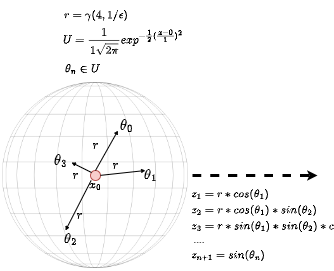
\includegraphics[width=0.6\textwidth]{TheorethicalFramework/ND-Laplace/Images/nd_laplace.png}
  \caption{Overview of the nD-Laplace mechanism}
  \label{fig:nd-laplace-overview}
\end{figure}
\newpage
\subsection{Privacy versus utility} \label{theory:privacy-utility-nd}
If we continue adding dimensions, we notice the noise is shrinking proportionally.
To understand this behavior, we first have to examine the formula for a hypersphere’s volume.
\begin{equation}
  S_n = \frac{2 \pi^{n/2}}{\gamma(\frac{1}{2}n)}
\end{equation}
Where $\gamma$ is the gamma distribution that is determined based on the number of dimensions $n$ \footnote{https://mathworld.wolfram.com/Hypersphere.html}.
As the amount of dimensions increases, the most volume is located on the hypersphere surface.
When we convert the points to Cartesian coordinates, some will be located at the center (e.g., 0.5), while others will be close to the surface (e.g., 0.0).
However, as the number of dimensions increases, the majority will be close to the surface (e.g., 0.99).
The decreasing amount of volume is illustrated using this figure:
\begin{figure}[ht]
  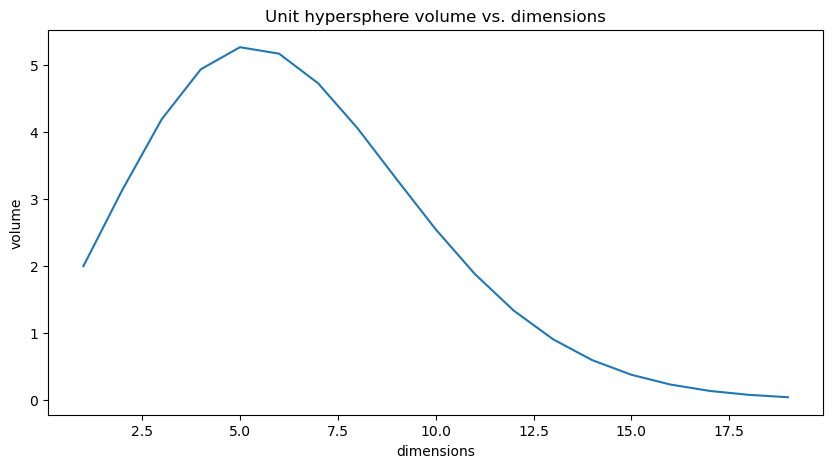
\includegraphics[width=0.8\textwidth]{TheorethicalFramework/ND-Laplace/Images/volume.png}
  \caption{Illustration of the decreasing volume while increasing the number of dimensions}
  \label{fig:curse-of-dimensionality}
\end{figure}

The noise is lower for higher dimensions, and therefore the utility increases.
It is therefore interesting to see how privacy behaves in comparison to utility.

\subsection{Truncation}
\todo[inline]{In progress}